Extra uitleg van een commando kan vaak ook gevonden worden door de optie -h of -{}-help aan het commando toe te voegen.

\begin{lstlisting}[language=bash]
$ mkdir -h
mkdir: invalid option -- 'h'
Try 'mkdir --help' for more information.
$ mkdir --help
Usage: mkdir [OPTION]... DIRECTORY...
Create the DIRECTORY(ies), if they do not already exist.

Mandatory arguments to long options are mandatory for short options too.
  -m, --mode=MODE   set file mode (as in chmod), not a=rwx - umask
  -p, --parents     no error if existing, make parent directories as needed,
                    with their file modes unaffected by any -m option.
  -v, --verbose     print a message for each created directory
  -Z                   set SELinux security context of each created directory
                         to the default type
      --context[=CTX]  like -Z, or if CTX is specified then set the SELinux
                         or SMACK security context to CTX
      --help        display this help and exit
      --version     output version information and exit

GNU coreutils online help: <https://www.gnu.org/software/coreutils/>
Full documentation <https://www.gnu.org/software/coreutils/mkdir>
or available locally via: info '(coreutils) mkdir invocation'
\end{lstlisting}

%\begin{figure}[H]
%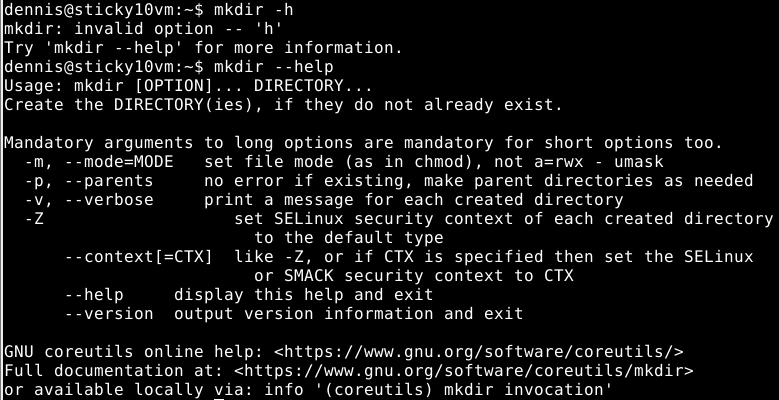
\includegraphics[width=0.8\linewidth]{linuxreader-img029.png}
%	\label{fig:DocHelp}
%	\caption{Gebruik van -h of --help}
%\end{figure}

In het voorgaande zie je dat -h een error melding geeft en ons vertelt dat we -{}-help moeten gebruiken. Ook wordt er verteld dat we de volledige documentatie kunnen vinden in de info-documentatie. Waarover later meer.

